\documentclass{beamer}

\mode<presentation>
{
  \usetheme{default}      % or try Darmstadt, Madrid, Warsaw, ...
  \usecolortheme{default} % or try albatross, beaver, crane, ...
  \usefonttheme{default}  % or try serif, structurebold, ...
  \setbeamertemplate{navigation symbols}{}
  \setbeamertemplate{caption}[numbered]
} 

\usepackage[english]{babel}
\usepackage[utf8]{inputenc}
\usepackage{filecontents}
% for subfigure :
\usepackage{graphicx}
\usepackage{caption}
\usepackage{subcaption}
% for algorithm :
\usepackage{varwidth}
\usepackage{verbatim}
\usepackage{algorithm}
\usepackage{algpseudocode}
% for algorithm
\newcommand{\vars}{\texttt}
\newcommand{\func}{\textrm}
\let\oldReturn\Return
\renewcommand{\Return}{\State\oldReturn}
% for demo animation :
\usepackage{animate}
\usepackage{multimedia}
%\begin{filecontents}{reference.bib}
%@article{donald1993kinodynamic,
%  title={Kinodynamic motion planning},
%  author={Donald, Bruce and Xavier, Patrick and Canny, John and Reif, John},
%  journal={Journal of the ACM (JACM)},
%  volume={40},
%  number={5},
%  pages={1048--1066},
%  year={1993},
%  publisher={ACM}
%}
%\end{filecontents}
%
%\usepackage[backend=bibtex]{biblatex}

\usepackage[style=verbose,autocite=footnote,maxnames=10,babel=hyphen,hyperref=true,abbreviate=false,backend=biber,mcite]{biblatex}
\addbibresource{reference.bib}

\makeatletter
\let\@@magyar@captionfix\relax
\makeatother

\title[Report]{Real-Time Kinodynamic Motion Planning for Omnidirectional Mobile Robot in Dynamic Environment with Moving Obstacles}
\author{Fahri Ali Rahman}
\institute{Department of Electrical Engineering and Information Technology}
\date{7 December 2018}

\begin{document}

\begin{frame}
  \titlepage
\end{frame}

% Uncomment these lines for an automatically generated outline.
%\begin{frame}{Outline}
%  \tableofcontents
%\end{frame}

\section{Introduction}

\begin{frame}{Introduction}

%\begin{itemize}
%  \item Kinodynamic motion planning problem : 
%  \item RoboCup MSL : example of highly dynamic and adversarial environment where moving obstacles and robot's dynamics are preferred to be taken into account.
%\end{itemize}
\begin{block}{\emph{Kinodynamic motion planning problem :}}
to plan robot motion subject to simultaneous kinematic and dynamic constraints 
%\footcite{donald1993kinodynamic} %% does not work, manual for now
\footnote{B. Donald, P. Xavier, J. Canny, and J. Reif, “Kinodynamic motion planning,” \emph{Journal of the ACM (JACM)}, vol. 40, no. 5, pp. 1048–1066, 1993.}
\end{block}

\vskip 1cm

\begin{block}{RoboCup MSL}
Example of highly dynamic and adversarial environment where moving obstacles and robot's dynamics are preferred to be taken into account.
\end{block}

\end{frame}

\begin{frame}{Research Objectives}
\begin{itemize}
\item generate a collision-free trajectory while satisfying kinodynamic constraint in environment that includes moving obstacles
\item implement trajectory tracking control to follows planned trajectory
\item develop software solution to enable online planning to address changing environment.
\end{itemize}
\end{frame}

\section{Method}

\begin{frame}{Motion Planning Strategy}
\begin{itemize}
\item separate planning in translational and rotational motion.
\item robot assumed as point with double integrator dynamics.
\item translational trajectory planned with kinodynamic-RRT*.
\item rotational trajectory planned with \emph{minimum-time trajectory generator}\footnote{O. Purwin and R. D’Andrea, “Trajectory generation and control for four wheeled omnidirectional vehicles,” \emph{Robotics and Autonomous Systems}, vol. 54, no. 1, pp. 13–22, 2006.}
\end{itemize}
\end{frame}

\subsection{Fixed-Final-State Free-Final-Time Optimal Control}

\begin{frame}{Fixed-Final-State Free-Final-Time Optimal Control for General Linear System}

\scalebox{0.8}{%
\begin{minipage}{1.2\textwidth}
$$
\dot{\mathbf{x}}=A\mathbf{x}+B\mathbf{u}
$$
\end{minipage}
}
with cost :
\scalebox{0.8}{%
\begin{minipage}{1.2\textwidth}
$$
c(\pi) = \int_{0}^{\tau}(1+\boldsymbol{u}(t)^{T}R\boldsymbol{u}(t))dt, \qquad R=Ir
$$
\end{minipage}
}
\vskip 0.25cm

solution trajectory \footnote{D. J. Webb and J. van den Berg, “Kinodynamic RRT*: Asymptotically optimal
motion planning for robots with linear dynamics,” in \emph{Robotics and Automation
(ICRA), 2013 IEEE International Conference on}. IEEE, 2013, pp. 5054–5061.}  :

\vskip 0.25cm
\scalebox{0.8}{
\begin{minipage}{1.2\textwidth}
$$
\begin{bmatrix}
\boldsymbol{x}(t)\\
\boldsymbol{y}(t)
\end{bmatrix}
=
e^{M(t-\tau^{*})}
\begin{bmatrix}
\boldsymbol{x}_f \\
\boldsymbol{d}(\tau^{*})
\end{bmatrix},
\quad
M = \begin{bmatrix}
A & BR^{-1}B^{T}\\
0 & -A^{T}
\end{bmatrix},
$$
$$
\boldsymbol{d}(\tau) = G(\tau)^{-1}(\boldsymbol{x}_f-\boldsymbol{\bar{x}}(\tau)),
\quad
\boldsymbol{\bar{x}}(t) = e^{At}\boldsymbol{x}_{i}.
$$
$$
\boldsymbol{u}(t) = R^{-1}B^{T}\boldsymbol{y}(t)
$$
\end{minipage}
}
\vskip 0.5cm
$\tau^{*} =$ optimal arrival time, $G =$ \emph{weighted controllability Gramian} \footnote{F. L. Lewis, D. Vrabie, and V. L. Syrmos, \emph{Optimal control}.
Sons, 2012.}

% Commands to include a figure:
%\begin{figure}
%\includegraphics[width=\textwidth]{your-figure's-file-name}
%\caption{\label{fig:your-figure}Caption goes here.}
%\end{figure}
\end{frame}

\begin{frame}{Fixed-Final-State Free-Final-Time Optimal Control for General Linear System}

To find Optimal Arrival Time \footnote{D. J. Webb and J. van den Berg, “Kinodynamic RRT*: Asymptotically optimal
motion planning for robots with linear dynamics,” in \emph{Robotics and Automation
(ICRA), 2013 IEEE International Conference on}. IEEE, 2013, pp. 5054–5061.}:

Cost :

$$
c(\tau) = \tau + (\boldsymbol{x}_f - \boldsymbol{\bar{x}}(\tau))^{T}G(\tau)^{-1}(\boldsymbol{x}_f-\boldsymbol{\bar{x}}(\tau))
$$

Derivative of cost :

$$
\dot{c}(\tau) = 1 - 2(A\boldsymbol{x}_f)^{T}\boldsymbol{d}(\tau)-\boldsymbol{d}(\tau)^{T}BR^{-1}B^{T}\boldsymbol{d}(\tau)
$$

to find optimal arrival time, solve $\dot{c}=0$ for $\tau$. \\
to solve the derivative of the cost : secant method.

\end{frame}

\subsection{Fixed-Final-State Free-Final-Time Optimal Control for Double Integrator Model}
\begin{frame}{Fixed-Final-State Free-Final-Time Optimal Control for Double Integrator Model}
\centering
\scalebox{0.7}{%
\begin{minipage}{1.2\textwidth}
$$
\dot{\boldsymbol{x}} = \begin{bmatrix}
0 & I \\
0 & 0
\end{bmatrix}\boldsymbol{x} + \begin{bmatrix}
0 \\
I
\end{bmatrix}\boldsymbol{u}
$$

$$
\begin{bmatrix}
\boldsymbol{x}(t)\\
\boldsymbol{y}(t)
\end{bmatrix}
=
\begin{bmatrix}
I &
A_1 & A_2 & A_3
\\
0 & I & A_4 & A_5 \\
0 & 0 & I & 0 \\
0 & 0 & A_6 & I
\end{bmatrix}
\begin{bmatrix}
\boldsymbol{x}_f\\
\boldsymbol{d}(\tau^{*})
\end{bmatrix}
$$

$$
A_1 = 
\begin{bmatrix}
t-\tau & 0 \\
0 & t-\tau
\end{bmatrix}
\quad
A_2 = 
\begin{bmatrix}
\frac{(-t+\tau)(t-\tau)^2}{6r} & 0 \\
0 & \frac{(-t+\tau)(t-\tau)^2}{6r}
\end{bmatrix}
\quad
A_3 = \begin{bmatrix}
\frac{(t-\tau)^2}{2r} & 0 \\
0 & \frac{(t-\tau)^2}{2r}
\end{bmatrix}
$$

$$
A_4 = \begin{bmatrix}
\frac{(-t+\tau)(t-\tau)}{2r} & 0 \\
0 & \frac{(-t+\tau)(t-\tau)}{2r}
\end{bmatrix} 
\quad
A_5 = \begin{bmatrix}
\frac{t-\tau}{r} & 0\\
0 & \frac{t-\tau}{r}
\end{bmatrix}
\quad
A_6 = \begin{bmatrix}
-t+\tau & 0 \\
0 & -t+\tau
\end{bmatrix}
$$

\emph{weighted controllability Gramian} :
$$
G(t)=\begin{bmatrix}
\frac{t^{3}}{3r} & 0 & \frac{t^{2}}{2r} & 0 \\
0 & \frac{t^{3}}{3r} & 0 & \frac{t^{2}}{2r} \\
\frac{t^{2}}{2r} & 0 & \frac{t}{r} & 0\\
0 & \frac{t^{2}}{2r} & 0 & \frac{t}{r}
\end{bmatrix}
,\quad
G^{-1}(t) =\begin{bmatrix}
\frac{12r}{t^{3}} & 0 & \frac{-6r}{t^{2}} & 0 \\
0 & \frac{12r}{t^{3}} & 0 & \frac{-6r}{t^{2}} \\
\frac{-6r}{t^{2}} & 0 & \frac{4r}{t} & 0 \\
0 & \frac{-6r}{t^{2}} & 0 & \frac{4r}{t}
\end{bmatrix}
$$
\end{minipage}
}

\end{frame}

\subsection{Collision Checking}
\begin{frame}{Line Circles Collision Check}
\begin{figure}
	\centering 
	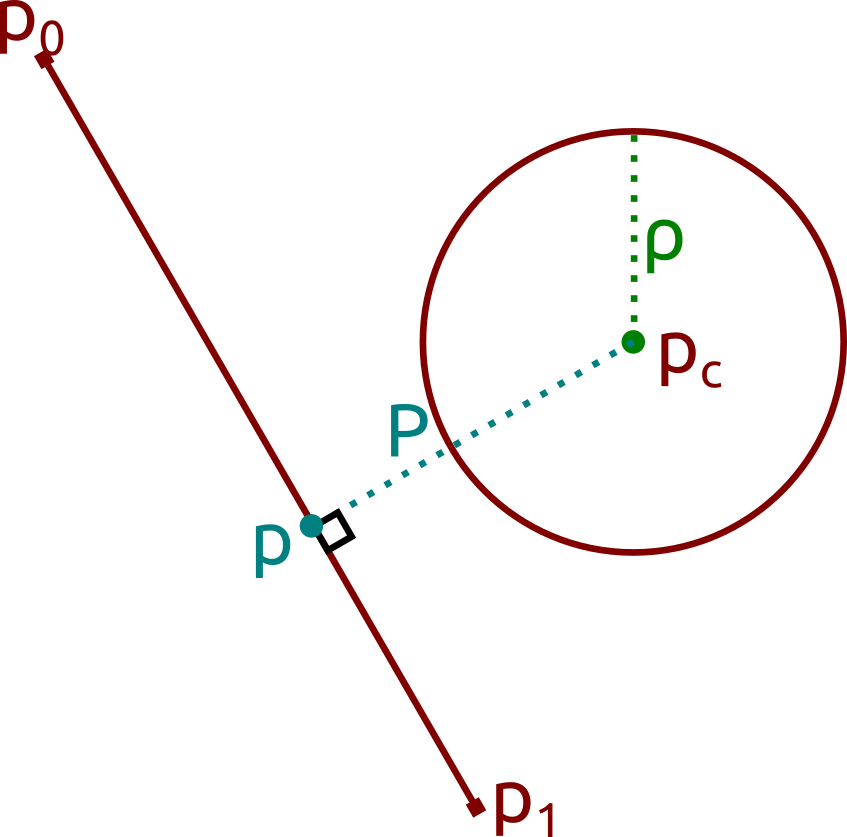
\includegraphics[width=0.35\linewidth]{assets/collision}
	\caption{Collision check for line and circle}
	\label{collision}
\end{figure}
\scalebox{0.75}{%
\begin{minipage}{1.2\textwidth}
$$
u = \frac{(c_x-p_{0x})(p_{1x}-p_{0x})+(c_y-p_{0y})(p_{1y}-p_{0y})}{\|p_1-p_0\|^2}
$$
$$
p \leftarrow p_{0} + u (p_{1}-p_{0})
,\quad
R = \|p3-c\|
$$
\end{minipage}
}
\vskip 0.25cm
Line and circle collide if $R<=r$.
\vskip 0.25cm
\end{frame}

\begin{frame}{Collision Checking for Trajectory and Moving Obstacles}
\centering
\scalebox{0.75}{%
\begin{minipage}{1.250\textwidth}
\begin{algorithm}[H]
\begin{algorithmic}[1]
\Function{TrajectoryCollision}{$\vars{trajectory}, \vars{DynamicObstacles}$}
	\For{$(x_0,y_0,x_1,y_1,t_0,t_1) \in \vars{trajectory}$}
		\State $\vars{Obstacles} \leftarrow \vars{DynamicObstacles} \;\func{at time}\; t_0 \;\func{and} \;t_1$
		\State $\vars{collision} = \textsc{LineCirclesCheck}(x_0,y_0,x_1,y_1,\vars{Obstacles})$
		\If{$\vars{collision}$}
			\Return {$\vars{True}$}
		\EndIf
	\EndFor
    \Return {$\vars{False}$}
\EndFunction
\end{algorithmic}
\caption{Trajectory Collision Checking with Moving Obstacles}
\label{trajectory_collision_alg}
\end{algorithm}
\end{minipage}%
}
\end{frame}

\subsection{Kinodynamic-RRT*}

\begin{frame}{Kinodynamic-RRT*}
\centering
\scalebox{0.5}{%
\begin{minipage}{1.50\textwidth}
\begin{algorithm}[H]
\begin{algorithmic}[1]
\Function{DoubleIntKinodynamic-RRT*}{$\boldsymbol{q}_{start}, \boldsymbol{q}_{goal}, p, n_{iter}$}
	\State $\mathcal{T} \leftarrow \{\boldsymbol{q}_{start}\}$
	\For{ $i\in [1,n_{iter}]$ }
		\State $\boldsymbol{q}_i \leftarrow \func{Sample}(\boldsymbol{q}_{goal})$
		\State $\boldsymbol{q}_{neighbor} \leftarrow \mathcal{T} \mid c^{*}(\boldsymbol{q},\boldsymbol{q}_i) < r \wedge \, not \,\textsc{TrajectoryCollision}(\pi^{*}(\boldsymbol{q},\boldsymbol{q}_i))$
		\State $\boldsymbol{q} \leftarrow \func{argmin} \left(\{ \boldsymbol{q} \in \boldsymbol{q}_{neighbor} \right\}(c^{*}(\boldsymbol{q},\boldsymbol{q}_i))$
		\State $parent(\boldsymbol{q}_i) \leftarrow \boldsymbol{q}$
		\State $cost(\boldsymbol{q}_i) \leftarrow cost(\boldsymbol{q}) + c^{*}(\boldsymbol{q},\boldsymbol{q}_i)$
		\State
			$\boldsymbol{q}_{neighbor} \leftarrow \mathcal{T} \cup \{q_{goal}\} \mid c^{*}(\boldsymbol{q}_i,\boldsymbol{q}) < r $
			\par\hskip\algorithmicindent $\wedge \, not \, \textsc{TrajectoryCollision}(\pi^{*}(\boldsymbol{q}_i,\boldsymbol{q}))$
			%\end{varwidth}
		\For{$\boldsymbol{q} \in \boldsymbol{q}_{neighbor}$}
			\If{$cost(\boldsymbol{q}_i)+c^{*}(\boldsymbol{q}_i,\boldsymbol{q})<cost(\boldsymbol{q})$}
				\State $parent(\boldsymbol{q}) \leftarrow \boldsymbol{q}_i$
				\State $cost(\boldsymbol{q}) \leftarrow cost(\boldsymbol{q}_i)+c^{*}(\boldsymbol{q}_i,\boldsymbol{q})$
			\EndIf
		\EndFor
		\If{$parent(q_i)$}
			\State $\mathcal{T}\leftarrow\mathcal{T}\cup q_i$
		\EndIf
	\EndFor
	\State $\boldsymbol{q}_{solution}[]\leftarrow\emptyset$
	\State $\boldsymbol{q}\leftarrow\boldsymbol{q}_{goal}$
	\While {$parent(\boldsymbol{q})$}
		\State $\func{insert}\;\pi^{*}(parent(\boldsymbol{q}),\boldsymbol{q})\; \func{to}\; \boldsymbol{q}_{solution}[]$
		\State $\boldsymbol{q}\leftarrow parent(\boldsymbol{q})$
	\EndWhile
	\Return $\boldsymbol{q}_{solution}[]$
\EndFunction
\end{algorithmic}
\caption{Implemented Kinodynamic-RRT* Algorithm}
\label{impl_rrt}
\end{algorithm}
\end{minipage}%
}
\end{frame}

\section{Motion Planning Strategy}

\subsection{Sampling Strategy}

\begin{frame}{Sampling Strategy}

Stochastic Decision to Directly Sampling the Goal State \footnote{J. Bruce and M. M. Veloso, “Real-time randomized path planning for robot
navigation,” in \emph{Robot Soccer World Cup. Springer}, 2002, pp. 288–295.} to improve the quality of solution trajectory. 

The stocastic decision decide wether or not to directly sampling the goal state:

\begin{itemize}
\item with probalility $p$, direcly sampling the goal state,
\item with probability $1-p$, randomly sample the state from uniform distribution.
\end{itemize}

\end{frame}

\section{Trajectory Tracking Strategy}
\begin{frame}{Trajectory Tracking for Omnidirectional Mobile Robot}
\begin{itemize}
\item PI-Trajectory Tracking for Omnidirectional Mobile  Robot \footnote{Y. Liu, J. J. Zhu, R. L. Williams II, and J. Wu, “Omni-directional mobile robot controller based on trajectory linearization,” \emph{Robotics and Autonomous Systems}, vol. 56, no. 5, pp. 461–479, 2008.} :
\vskip 0.25cm
\scalebox{0.8}{%
\begin{minipage}{1.2\textwidth}
$$
\begin{bmatrix}
\tilde{u} \\ \tilde{v} \\ \tilde{r}
\end{bmatrix} = 
-K_{P}
\begin{bmatrix}
e_x \\ e_y \\ e_{\omega}
\end{bmatrix}
-K_{I}
\begin{bmatrix}
\int e_x(t)dt \\
\int e_y(t)dt \\
\int e_{\omega}(t)dt
\end{bmatrix}
$$

$$
K_{I} = 
-B_{1}^{-1} 
\begin{bmatrix}
-a_{I1} & 0 & 0 \\
0 & -a_{I2} & 0 \\
0 & 0 & -a_{I3}
\end{bmatrix}
,\quad
K_{P} = 
-B_{1}^{-1} 
( A_1 - 
\begin{bmatrix}
-a_{P1} & 0 & 0 \\
0 & -a_{P2} & 0 \\
0 & 0 & -a_{P3}
\end{bmatrix}
)
$$
\end{minipage}
}
\end{itemize}
\end{frame}

\section{Numerical Experiment}
\subsection{Translational Trajectory}
\begin{frame}{Numerical Experiment : Translational Trajectory}
\begin{figure}[H]
	\centering
	\begin{subfigure}{0.4\textwidth}
		\centering
		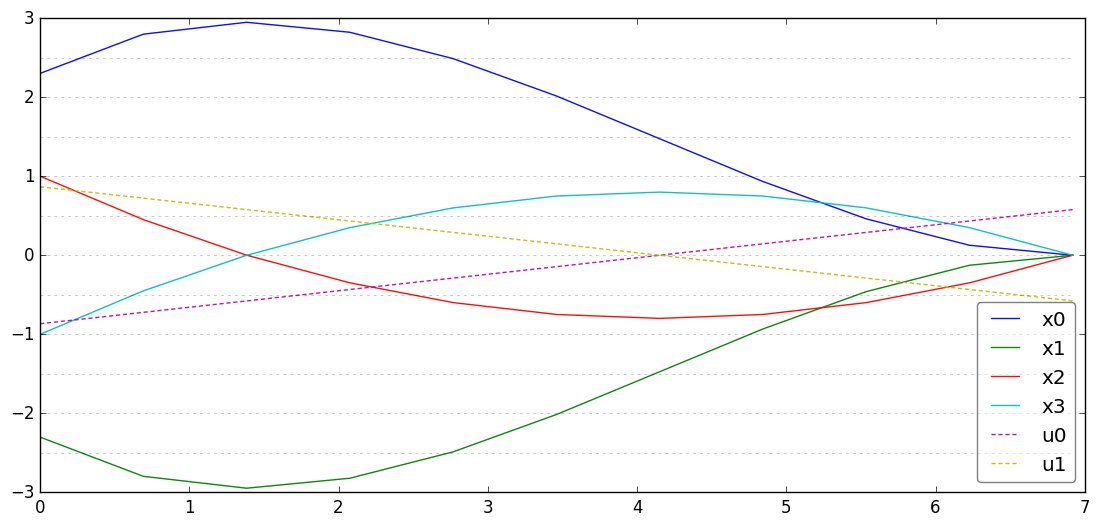
\includegraphics[width=1.0\linewidth]{assets/fig1}
		\caption{Double Integrator Trajectory with $r=1.5$.}
		\label{trajectory1}
	\end{subfigure}
	\begin{subfigure}{0.4\textwidth}
		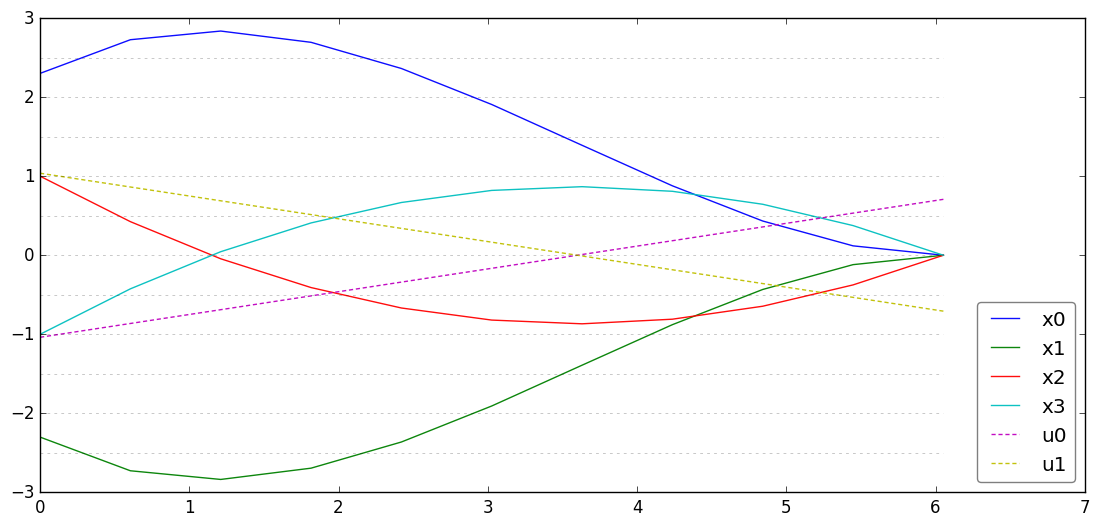
\includegraphics[width=1.0\linewidth]{assets/fig2}
		\caption{Double Integrator Trajectory with $r=1.0$.}
		\label{trajectory2}
	\end{subfigure}
	\begin{subfigure}{0.4\textwidth}
		\centering
		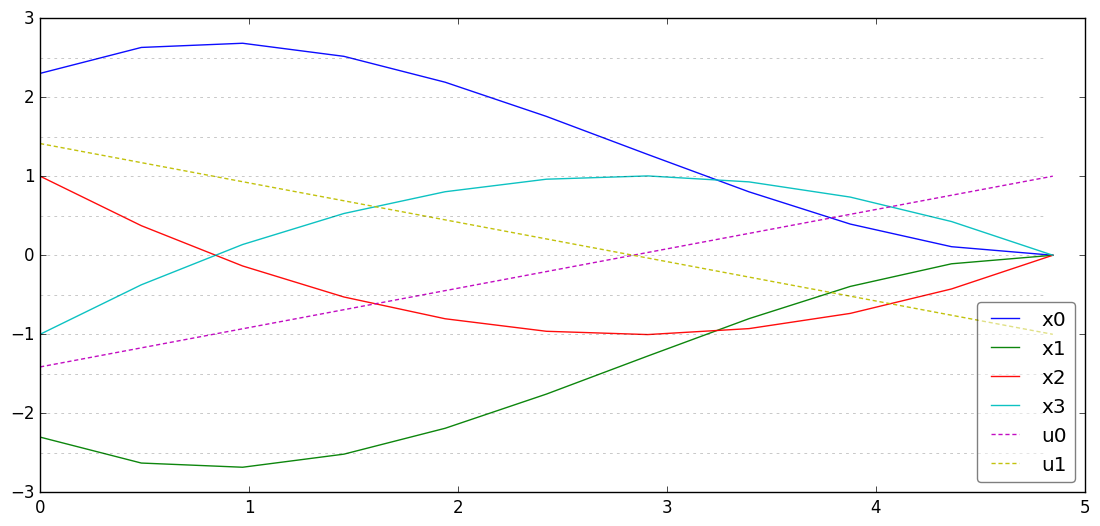
\includegraphics[width=1.0\linewidth]{assets/fig3}
		\caption{Double Integrator Trajectory with $r=0.5$.}
		\label{trajectory3}
	\end{subfigure}
\end{figure}
\end{frame}

\begin{frame}{Numerical Experiment : Translational Trajectory}
\begin{table}[]
\caption{Arrival Time and Maximum Control Input for Several Input Weight}
\label{trajectories_table}
\centering
\begin{tabular}{|l|l|l|}
\hline
$r$ & arrival time (s) & maximum $\| u \| \; (m/s^2)$ \\ \hline
$1.5$ & $6.9187936337$ & $1.2253000912634624$ \\ \hline
$1.0$ & $6.05276367644$ & $1.467295152420136$ \\ \hline
$0.5$ & $4.84707681233$ & $1.997746119057331$ \\ \hline
\end{tabular}
\end{table}
\end{frame}

\subsection{Rotational Trajectory}
\begin{frame}{Numerical Experiment : Rotational Trajectory}
\begin{table}[ht]
\caption{Arrival Time}
\label{arrival_time}
\centering
\resizebox{\columnwidth}{!}{%
\begin{tabular}{|l|l|l|l|}
\hline
Exp. No. & Constraints $[\dot{\omega}_{max}\,, \ddot{\omega}_{max}\,]$ & Trajectory $max(\|\dot{\omega}\| []),, max(\|\ddot{\omega}\|[])$ & arrival time ($s$) \\ \hline
$1$.     & $[0.5\;rad/s;\;0.5\;rad/s^2]$ & $[1.0\;rad/s;\;0.5\;rad/s^2]$ & $4.6$              \\ \hline
$2$.     & $[1.0\;rad/s;\;1.0\;rad/s^2]$ & $[1.0\;rad/s;\;1.0\;rad/s^2]$ & $2.8$              \\ \hline
$3$.     & $[1.5\;rad/s;\;1.5\;rad/s^2]$ & $[1.5\;rad/s;\;1.5\;rad/s^2]$ & $2.08889$          \\ \hline
\end{tabular}
}
\end{table}
\end{frame}

\subsection{Kinodynamic-RRT*}

\begin{frame}{Numerical Experiment : Computation Time for Kinodynamic-RRT*}
\begin{figure}[H]
	\centering
	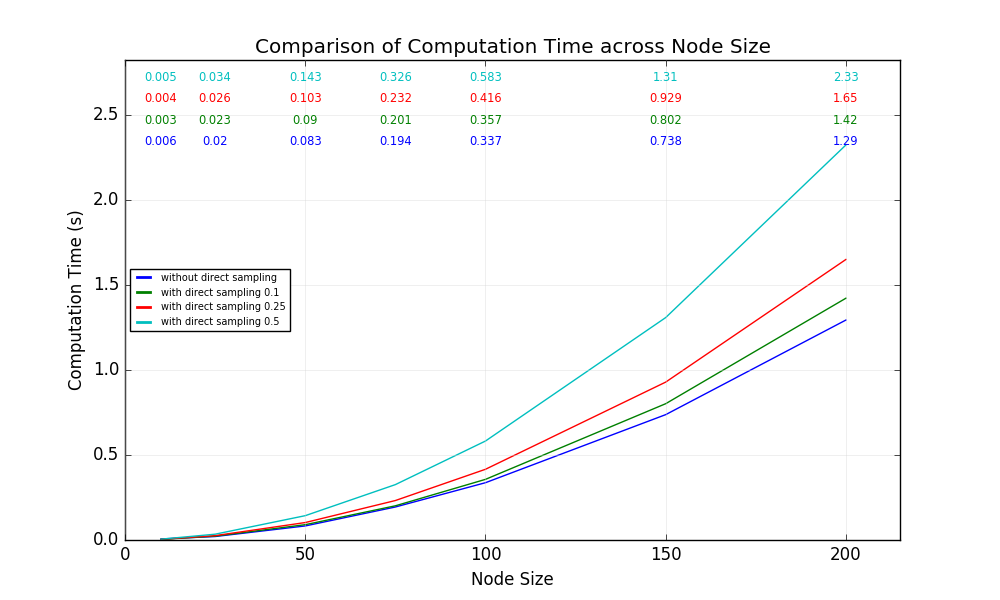
\includegraphics[width=\linewidth]{assets/plot_time_all}
	\caption{The Computation Time to grow the Tree}
	\label{plot_compare_all:time}
\end{figure}
\end{frame}

\begin{frame}{Numerical Experiment : Solution Cost}
\begin{figure}[H]
	\centering
	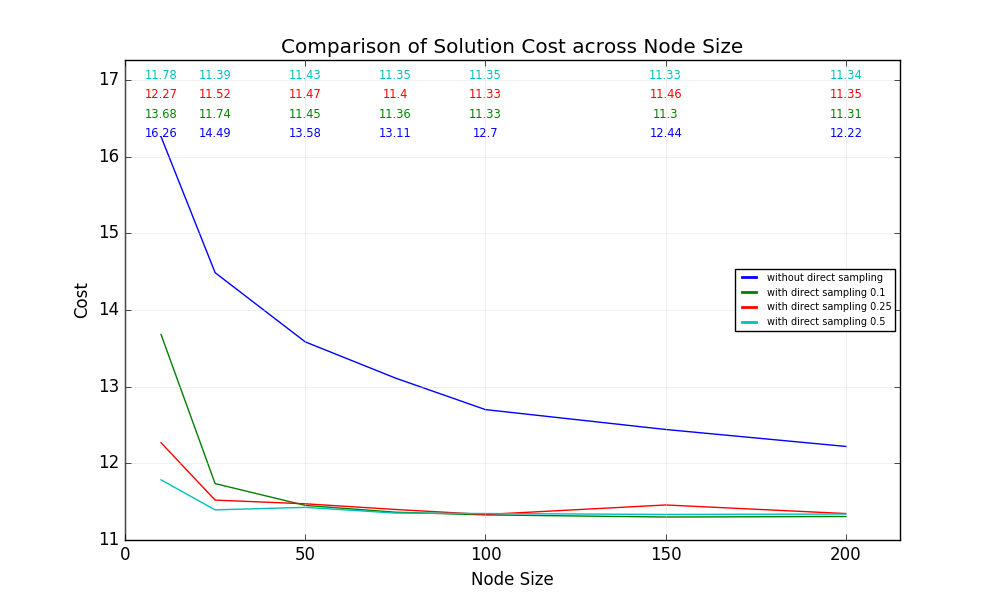
\includegraphics[width=\linewidth]{assets/plot_cost_all}
	\caption{The Solution Cost of the Tree}
	\label{plot_compare_all:cost}
\end{figure}
\end{frame}

\begin{frame}{Numerical Experiment : Solution Cost}
\centering
\scalebox{1.075}{%
\centering
\begin{minipage}{1.0\textwidth}
\centering
\begin{figure}
	\centering
	\begin{subfigure}{0.485\textwidth}
		\centering
		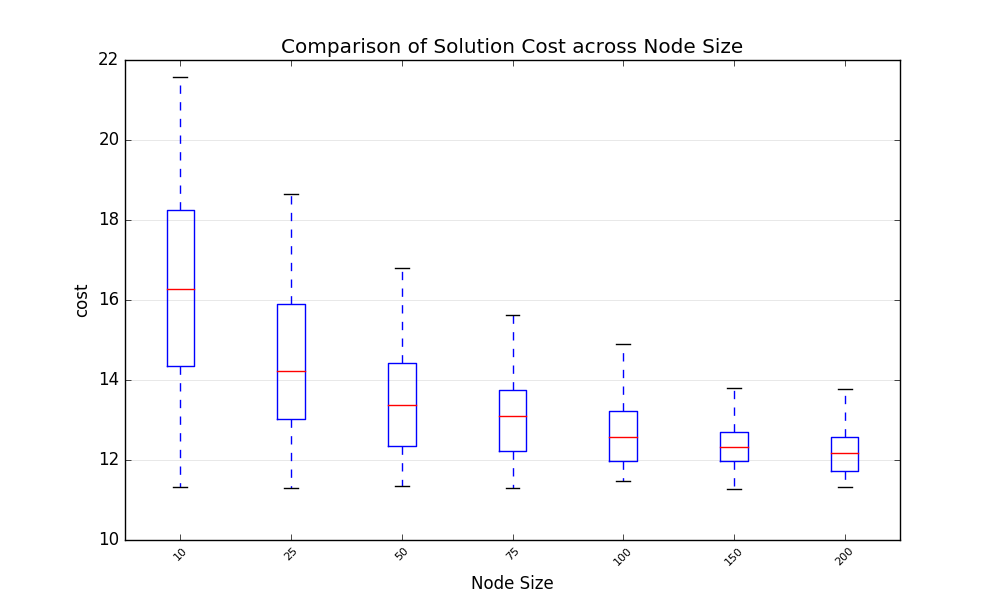
\includegraphics[width=1\linewidth]{assets/boxplot_cost_no}
%		\caption{Solution Cost without Direct Sampling}
%		\label{plot_compare_cost:no}
	\end{subfigure}
	\begin{subfigure}{0.485\textwidth}
		\centering
		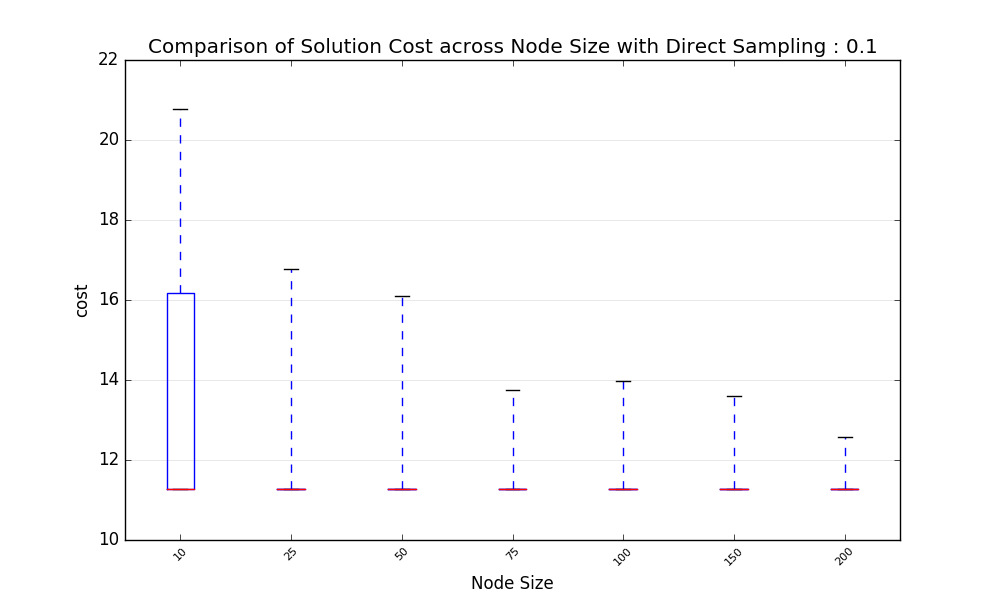
\includegraphics[width=1\linewidth]{assets/boxplot_cost_01}
%		\caption{Solution Cost without Direct Sampling with $p=0.1$}
%		\label{plot_compare_cost:0.1}
	\end{subfigure}
	\caption{Comparison of Solution Cost without and with Direct Sampling}
	\label{plot_compare_cost}
\end{figure}
\end{minipage}
}
\end{frame}


\section{Dynamic Simulation Experiment}

\begin{frame}{Online Planning \& Tracking}

\centering
\scalebox{0.8}{%
\begin{minipage}{1.\textwidth}
\begin{figure}
	\centering
	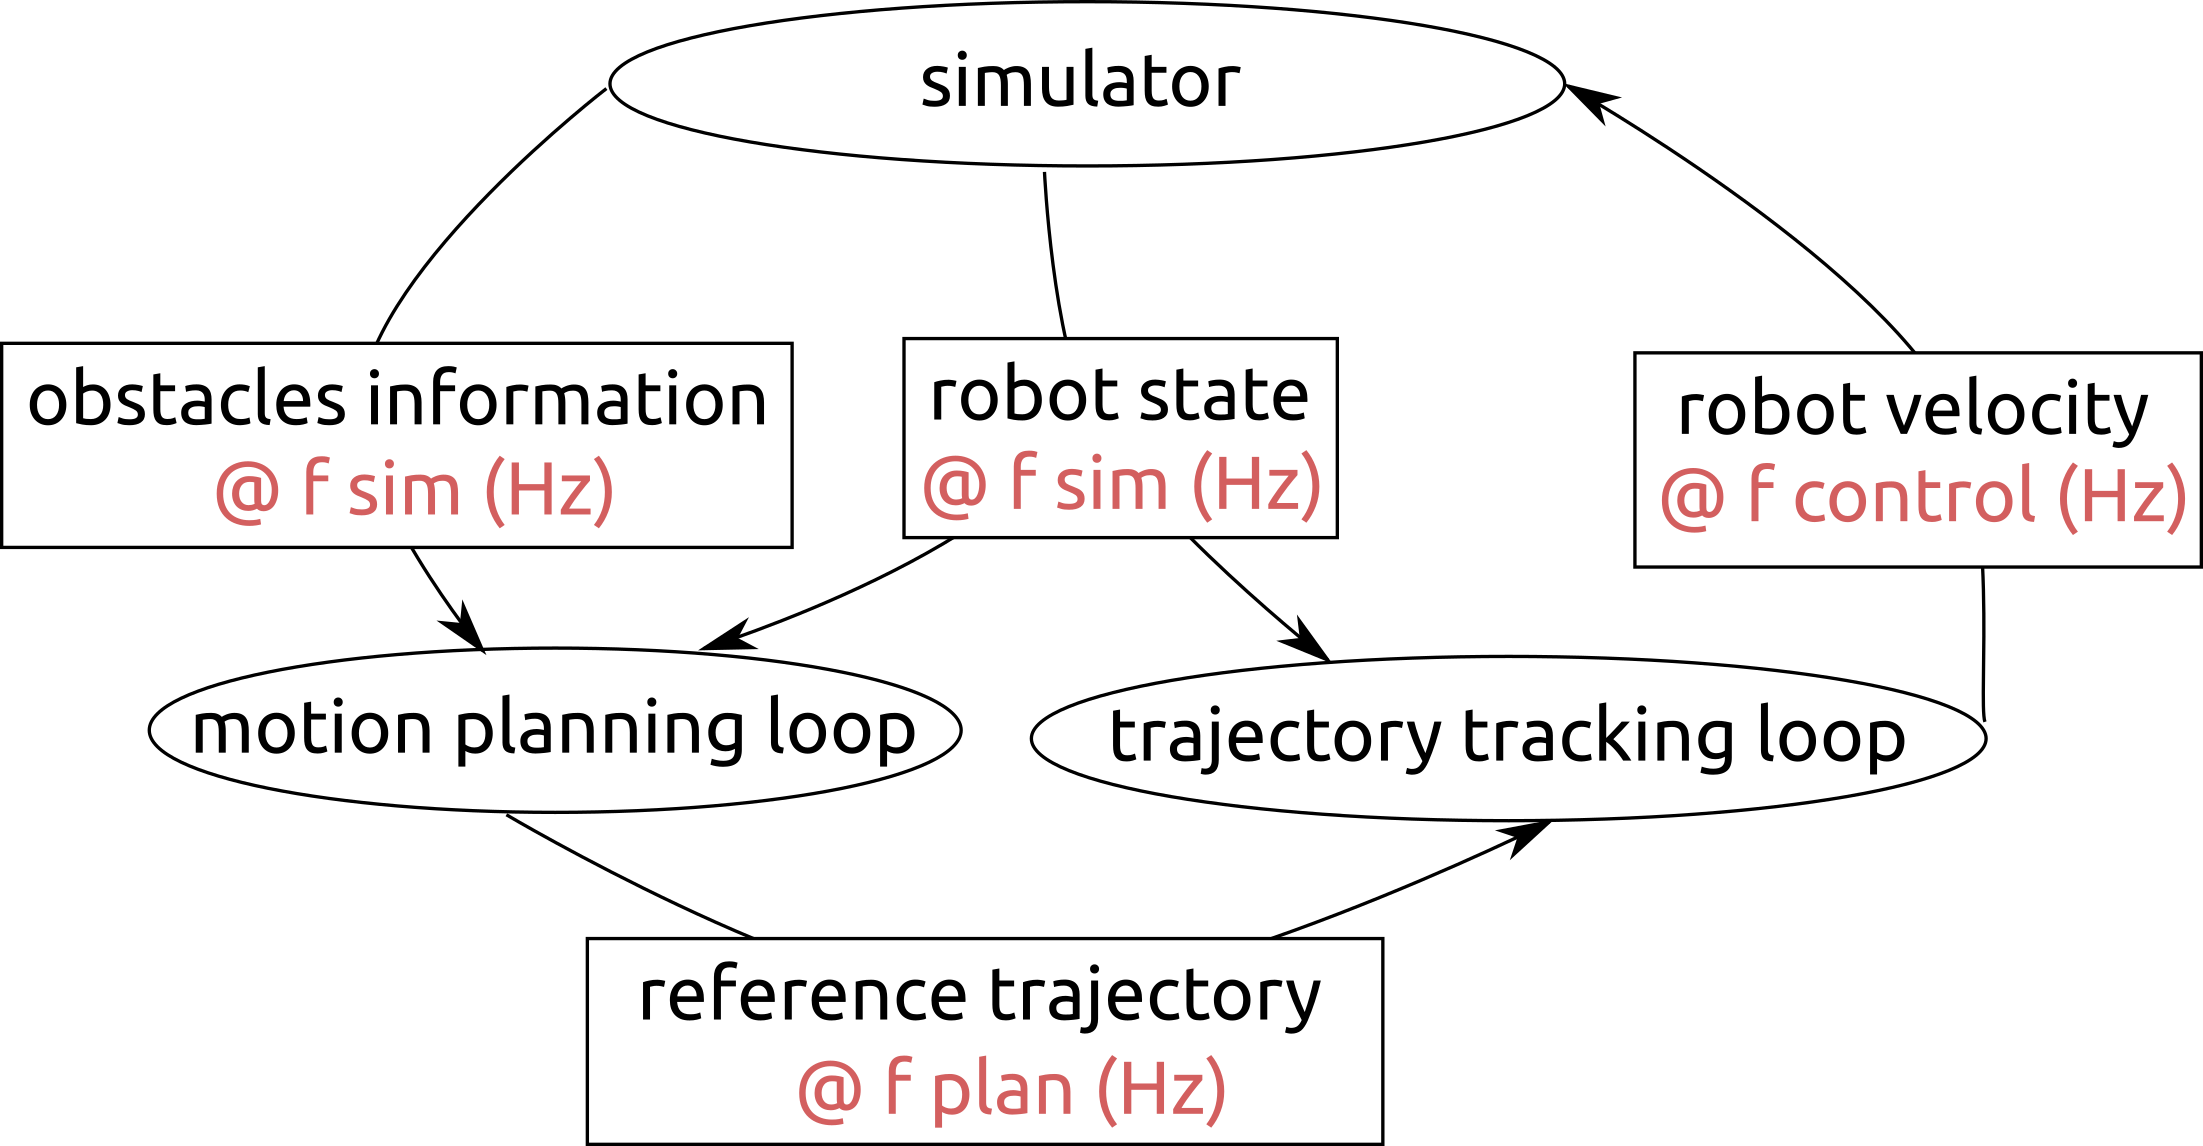
\includegraphics[width=1\linewidth]{assets/online_loop}
	\caption{Online Computation of Motion Planning and Trajectory Tracking}
	\label{online_loop}
\end{figure}
\end{minipage}
}%

\begin{itemize}
\item ROS-based
\item Message exchange between module
\item concurrent execution
\end{itemize}

\end{frame}

\begin{frame}{Dynamic Simulation Experiment}

ROS-Based simulation framework \footnote{W. Yao, W. Dai, J. Xiao, H. Lu, and Z. Zheng, “A simulation system based on ros and gazebo for robocup middle size league,” in \emph{Robotics and Biomimetics (ROBIO), 2015 IEEE International Conference on}. IEEE, 2015,
pp. 54–59.}.

Source code of the implemented algorithm : \url{bitbucket.org/alifahrri/robosoccer_motion_planning_ws}

\vskip 0.25cm
\centering
\scalebox{0.7}{%
\centering
\begin{minipage}{1.0\textwidth}
\centering
%\movie[height = 0.6 \textwidth,width = 1.0 \textwidth]{}{demo/demo_short2.mp4}
\animategraphics[loop,controls,width=\linewidth]{10}{demo/demo_short-}{0}{25}
\end{minipage}
}

\end{frame}

\section{Conclusion and Future Works}

\begin{frame}{Conclusion}
\begin{itemize}
\item \emph{Kinodynamic motion planning} for omnidirectional mobile robot was presented.
\item Obstacles' motion was taken into account while planning the trajectory.
\item Dynamic constraints for translational motion was addressed by penalizing control input while dynamic constraints for rotational motion was satisfied by setting maximum allowed velocity and acceleration.
\item The presented sampling strategy was able to reduce solution cost.
\item Online planning \& tracking scheme was presented.
\item Dynamic simulation shows the scheme was successfully applied to the simulated robot and environment.
\end{itemize}
\end{frame}

\begin{frame}{Future Works}
\scalebox{0.9}{%
\begin{minipage}{1.10\textwidth}
\begin{itemize}
\item \emph{synchronize} motion in translation and rotation by taking the robot's motion in body frame into account.
\item take subsequent reference pose into account while tracking the reference trajectory, e.g. using Model Predictive Controller.
\item develop a robot localization system and also obstacles' detection and tracking may be developed to implements this work in real robot.
\item take the \emph{uncertainty} of robot's and obstacles' state into account while solving the trajectory, e.g. motion planning under uncertainty.
\item increase the quality of solution trajectory and computation efficiency by implement \emph{heuristic} for the sampling procedure.
\end{itemize}
\end{minipage}%
}
\end{frame}

\end{document}